\section{Étude du bras manipulateur}
 Le package scientifique équipant ROBOVOLC est formé d'un bras manipulateur et d'une pince
 servant d'effecteur pour collecter des échantillons rocheux et poser/prendre des instruments sur le
 sol. Ces organes sont pilotés par des moteurs à courant continu contrôlés par des modules
 électroniques. Le système est en outre constitué d'un système d'échantillonnage des gaz (avec
 sonde) qui ne sera pas étudié ici. 
 
 \begin{obj}
 L'objectif de cette partie est de valider les performances de déplacement multidirectionnel
 du bras manipulateur et de vérifier leur compatibilité avec le critère suivant du cahier des
 charges.
 
 \begin{center}
 \begin{tabular}{ll}
 \textbf{Critère} & \textbf{Valeur} \\
Masse maximale des objets à saisir & $\SI{2,5}{kg}$ \\
 \end{tabular}
 \end{center}
 \end{obj}
 
 \subsection{Modélisation cinématique}
\textbf{ Dans cette sous-partie, on établit le lien entre la cinématique des liaisons et la cinématique
 de la pince située au bout du bras. }
 
Le bras manipulateur est de type SCARA (\textit{Selective Compliance Assembly Robot Arm}); c'est un
 système mécanique poly-articulé avec trois axes parallèles et une architecture en série (Figure
 \ref{xens_2027_fig20}). Il présente plusieurs avantages, notamment sa précision, sa rapidité, et sa très grande rigidité verticale. 
L'ensemble est constitué de trois pièces assimilées à des solides indéformables :
\begin{itemize}
\item le bras 1, de masse $m_1$, auquel on associe un repère $\repere{O_1}{x_1}{y_1}{z_1}$;
\item le bras 2, de masse $m_2$, auquel on associe un repère $\repere{O_2}{x_2}{y_2}{z_2}$;
\item la tige 3 au bout de laquelle se situe la pince et éventuellement l'objet saisi. La masse $m_3$ de ce
 sous-ensemble est supposée ponctuelle au point $P$ correspondant à la position de la pince.
 \end{itemize}
 Dans cette étude, le châssis de ROBOVOLC constitue le bâti 0 auquel on associe un repère (fixe)
 $\repere{O_0}{x_0}{y_0}{z_0}$. On suppose par la suite que le sol est plan et horizontal ; la direction $\vz{0}=\vz{1}=\vz{2}$
 correspond donc à la verticale. On suppose également que le référentiel lié au bâti est galiléen.
 
 Le positionnement horizontal de la pince dans le plan $\left(O_0,\vx{0},\vy{0}\right)$ est obtenu par deux rotations indépendantes : 
 \begin{itemize}
 \item celle du bras 1 en liaison pivot d'axe $\axe{O_1}{z_0}$ par rapport au bâti 0, on note $\theta_1 = \angle{x_0}{x_1}$ l'angle correspondant ;
 \item celle du bras 2 en liaison pivot d'axe $\axe{O_2}{z_0}$ par rapport au bras 1, on note $\theta_2 = \angle{x_1}{x_2}$ l'angle correspondant.
 \end{itemize}
 
Le positionnement vertical de la pince est quant à lui obtenu par une liaison glissière de direction
 $\vz{0}$ entre la tige 3 et le bras 2. 
Toutes les liaisons sont supposées parfaites.
On note : $\vect{O_0O_1} = d_1 \vz{0}$, 
$\vect{O_1O_2} = l_1 \vx{1}+d_2 \z{0}$, 
$\vect{O_2 P} =l_2\vx{2} - \lambda_3 \vz{0}$.

Les 3 degrés de liberté du bras sont donc $\theta_1$, $\theta_2$ et $\lambda_3$. Le débattement permis pour les deux iaisons pivot est $\pm 150\degres$ (limitation par des butées). 
Un schéma cinématique du système est proposé sur la Figure \ref{xens_2027_fig20}.
 On donne de plus :
 $d_1 =\SI{500}{mm}$, $d_2 =\SI{30}{mm}$, $l_1=\SI{500}{mm}$, $l_2 =\SI{500}{mm}$, 
$m_1 =\SI{2}{kg}$, $m_2=\SI{2}{kg}$, $m_3 =\SI{6}{kg}$ (incluant un objet saisi de masse \SI{2,5}{kg}).

\begin{figure}[!h]
\centering
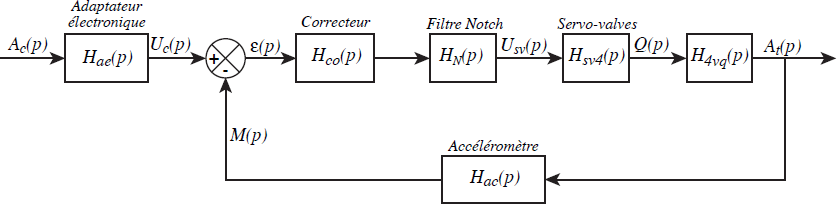
\includegraphics[width=.9\linewidth]{fig_20}
\caption{Schématisation et paramétrage du système SCARA \label{xens_2027_fig20}}
\end{figure}




 Dans un modèle cinématique direct, les données d'entrée sont les valeurs des angles de rotation
$\theta_1$ et $\theta_2$ (appelés variables articulaires) et de la position verticale $\lambda_3$ de la pince. On cherche alors la configuration du système à partir de ces variables. 

%Q4.1 : 
\question{En représentant sur le document réponse DR3 figure \ref{xens_2027_dr03} la base du cylindre, montrer que le volume accessible par le point $P$ (enveloppe de travail) est un cylindre à base non-circulaire. }
  \ifprof
 \begin{corrige}
 \begin{center}
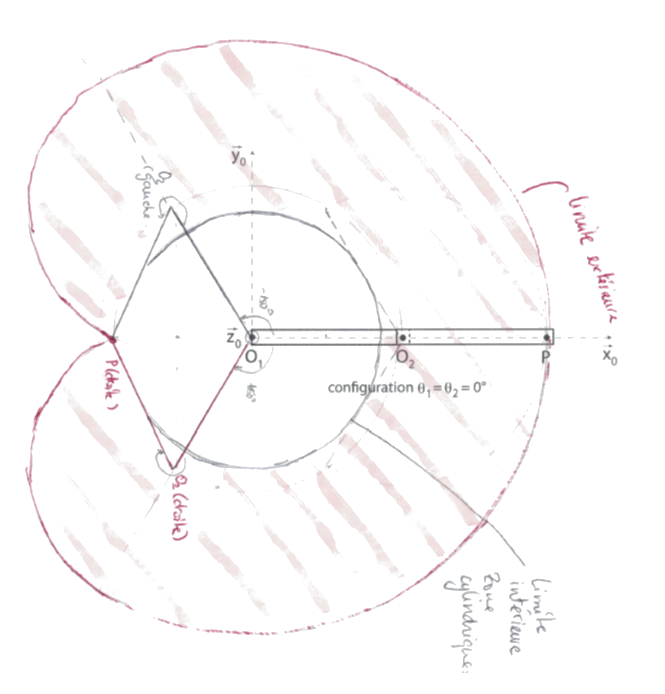
\includegraphics[width=.7\linewidth]{q_42_cor}
\end{center}
 \end{corrige}
 \else
 \fi
 
\begin{figure}[!h]
\centering
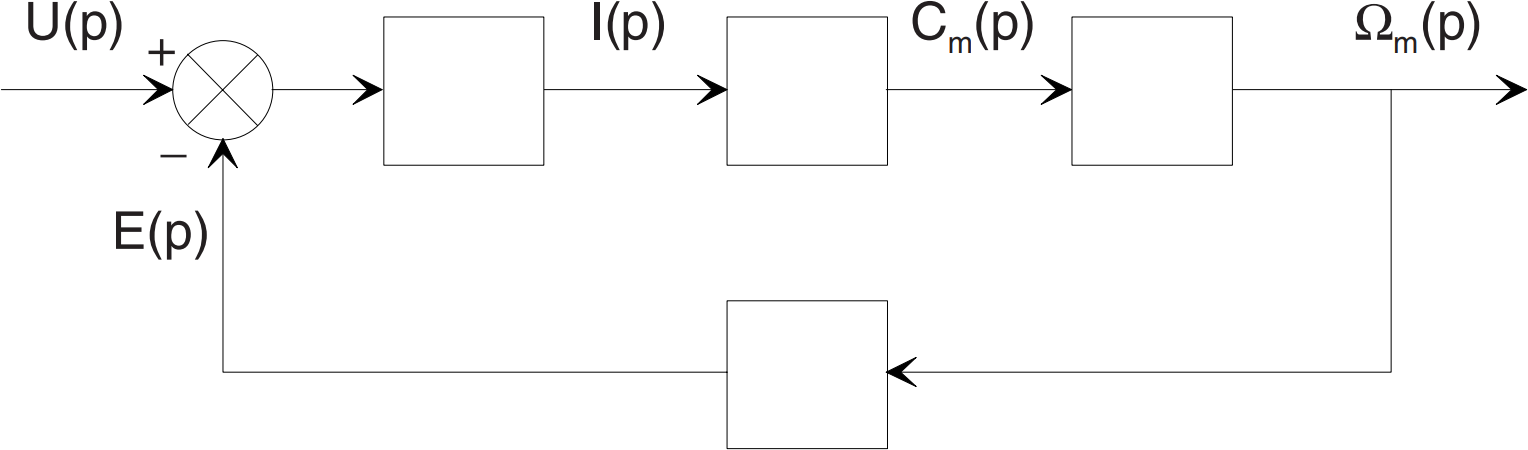
\includegraphics[width=.9\linewidth]{dr_03}
\caption{DR 3 \label{xens_2027_dr03}}
\end{figure}

%Q4.2 : 
\question{Donner l'expression des coordonnées $\left( x_P, y_P, z_P\right)$ et de la vitesse $\vectv{P}{3}{0}$
 du point $P$  dans le repère fixe $\repere{O_0}{x_0}{y_0}{z_0}$ en fonction des variables $\theta_1$, $\theta_2$, $\lambda_3$ et des dimensions constantes du problème. }
 \ifprof
 \begin{corrige}
 On a : 
 $\left\{
 \begin{array}{l}
 x_P = \ell_1 \cos \theta_1 + \ell_2 \cos(\theta_1 + \theta_2) \\
 y_P = \ell_1 \sin \theta_1 + \ell_2 \sin(\theta_1 + \theta_2) \\
 z_P = d_1 + d_2 - \lambda_3
  \end{array}
 \right.
 $
 
De plus : 
$\vectv{P}{3}{0} = \deriv{\vect{O_OO_3}}{\rep{0}} = \ell_1\thetap_1 \vy{1} + \ell_2\left( \thetap_1+\thetap_2\right)\vy{2}-\lambdap_3 \vz{0}$.
 \end{corrige}
 \else
 \fi
 
%Q4.3 : 
\question{Montrer que la vitesse maximale $\indice{V}{max}$ (en norme) que peut atteindre le point $P$ dans le
 plan $\left(O_0,\vx{0},\vy{0}\right)$ est obtenue pour $\theta_2 = 0\degres$. Exprimer $\indice{V}{max}$ en fonction de la vitesse de rotation maximale $\indice{\omega}{max}$ des moteurs et des dimensions constantes.}
  \ifprof
 \begin{corrige}
On exprime $\vectv{P}{3}{0}$ dans la base 1 par exemple et on calcule la norme de ce vecteur vitesse.

On obtient :
$||\vectv{P}{3}{0}|| = \sqrt{\ell_1^2\thetap_1^2 + \ell_2^2\left( \thetap_1+\thetap_2\right)^2+2\ell_1\thetap_1 \ell_2\left( \thetap_1+\thetap_2\right)\cos\theta_2+\lambdap_3 ^2  }$

$\lambdap_3 = 0$ car on considère ci un mouvement plan.

La vitesse du point $P$ est maximale lorsque $\theta_2=0\degres$, donc lorsque les deux bras sont alignés.
$||\vectv{P}{3}{0}|| = \sqrt{\ell_1^2\thetap_1^2 + \ell_2^2\left( \thetap_1+\thetap_2\right)^2+2\ell_1\thetap_1 \ell_2\left( \thetap_1+\thetap_2\right) }$
$ = \ell_1\thetap_1 + \left( \ell_1+\ell_2\right)\thetap_2$.

Dans ce cas, on a $\indice{V}{max}  =\ell_1\indice{\omega}{max} + \left( \ell_1+\ell_2\right)\indice{\omega}{max} =  \left( 2\ell_1+\ell_2\right)\indice{\omega}{max}$.

 \end{corrige}
 \else
 \fi
 
 Dans un modèle cinématique inverse, les données d'entrée sont la position $\left(x_P, y_P, z_P\right)$ et la
 vitesse $\left(V_P^x,V_P^y,V_P^z\right)$ de la pince située en $P$ dans le repère fixe $\repere{O_0}{x_0}{y_0}{z_0}$. On cherche  alors les lois à appliquer au niveau des liaisons (variables $\theta_1$, $\theta_2$, $\lambda_3$) pour obtenir ces données.

% Q4.4 : 
\question{Donner l'expression de $\lambda_3$  et $\lambdap_3$ en fonction de $z_P$ , $V_P^z$ et des dimensions constantes.}
 \ifprof
 \begin{corrige}
 $\lambda_3 = d_1 + d_2 -z_P$ et  $\lambdap_3 = -\dot{z}_P = -V_P^Z$.
 \end{corrige}
 \else
 \fi
 
% Q4.5 : 
\question{Pour une même position $\left(x_P, y_P, z_P\right)$ du point $P$ , montrer schématiquement qu'il y a deux configurations possibles des angles $\theta_1$ et $\theta_1$. Par un raisonnement graphique, donner sur le document DR4 figure \label{xens_2027_dr04} la configuration complémentaire de celle dessinée correspondant à $\theta_1 = 90\degres$ et $\theta_2 = -60\degres$.}
 \ifprof
 \begin{corrige}
 \end{corrige}
 \else
 \fi
 
\begin{figure}[!h]
\centering
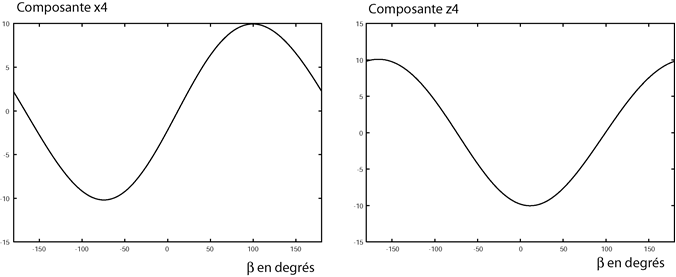
\includegraphics[width=.9\linewidth]{dr_04}
\caption{DR 4 \label{xens_2027_dr03}}
\end{figure}


% Q4.6 : 
\question{Montrer que quelle que soit la configuration, la valeur de l'angle $\theta_2$ est entièrement
 déterminée par $x_P^2 + y_P^2$ et donner l'expression de $\theta_2$ en fonction de $x_P^2 + y_P^2$ et des dimensions  constantes.}
  \ifprof
 \begin{corrige}
 \end{corrige}
 \else
 \fi
 
 \subsection{Modélisaton dynamique}
\textbf{Dans cette sous-partie, on construit un modèle dynamique du bras manipulateur.}

On suppose que chaque bras $i$ peut être modélisé géométriquement par un parallélépipède
 rectangle de génératrice $\vx{i}$ et à base carrée dans les directions $\vy{i}$ et $\vz{i}$ (Figure \ref{xens_2027_fig20}). On
 suppose de plus que le bras est homogène; son centre de gravité $G_i$ correspond donc au centre
 géométrique avec $\vect{O_iG_i} \dfrac{l_i}{2} \vx{i}$.
 

\begin{figure}[!h]
\centering
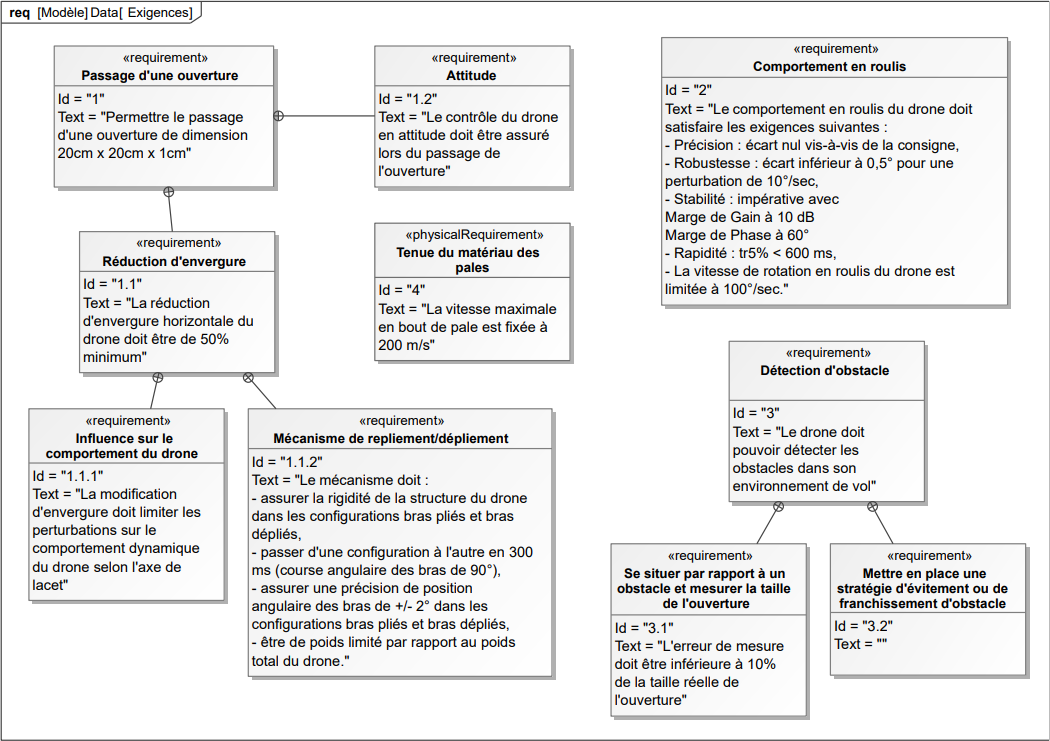
\includegraphics[width=.6\linewidth]{fig_21}
\caption{Modèle géométrique d'un bras \label{xens_2027_fig21}}
\end{figure}


On donne l'écriture générale de la matrice d'inertie du bras $i$ au point $G_i$ : 
$\inertie{i}{G_i} = \matinertie{A_i}{B_i}{C_i}{D_i}{E_i}{F_i}{\left( \vx{i},\vy{i},\vz{i}\right)}$.



 %Q4.7 : 
 \question{A partir de l'expression générale précédente, préciser et justifier la forme simplifiée de la
 matrice d'inertie $\inertie{i}{G_i}$ du bras $i$ prenant en compte sa modélisation géométrique.}
  \ifprof
 \begin{corrige}
 \end{corrige}
 \else
 \fi
 
 %Q4.8 : 
 \question{Déterminer l'hyperstatisme du modèle du système (Figure 20). Conclure sur la possibilité
 d'obtenir les différentes actions de liaison (leur calcul n'est pas demandé).}
 \ifprof
 \begin{corrige}
 \end{corrige}
 \else
 \fi
 
%Q4.9 : 
\question{Calculer les vitesses  $\vectv{G_i}{i}{0}$ et accélérations $\vectg{G_i}{i}{0}$ des points $G_1$ et $G_2$ dans leur mouvement par rapport au bâti 0, ainsi que $\vectv{P}{i}{0}$ et $\vectg{P}{i}{0}$, en fonction des
 paramètres variables ($\theta_1$, $\theta_2$, $\lambda_3$) et des dimensions constantes.}
  \ifprof
 \begin{corrige}
 \end{corrige}
 \else
 \fi
 